\newpage
{\bfseries МРНТИ 65.63.03}
\hfill {\bfseries \href{https://doi.org/10.58805/kazutb.v.2.23-447}{https://doi.org/10.58805/kazutb.v.2.23-447}}

\sectionwithauthors{Н.К. Турганбаева, Р.Ш. Элеманова, Н.С. Дюшеева}{К ВОПРОСУ ХАРАКТЕРИСТИКИ МОЛОКА ОСЛИЦ КЫРГЫЗСКОЙ ПОПУЛЯЦИИ}

\begin{center}
{\bfseries \textsuperscript{1}Н.К. Турганбаева, \textsuperscript{2}Р.Ш. Элеманова, \textsuperscript{2}Н.С. Дюшеева}

\textsuperscript{1}Кыргызско-Турецкий университет Манас, Бишкек,
Кыргызстан,

\textsuperscript{2}Кыргызский государственный технический университет
им. И. Раззакова, Бишкек, Кыргызстан

Корреспондент-автор: nadira.turganbaeva@manas.edu.kg
\end{center}

В статье затрагивается тема изучения альтернативного вида молока
обладающее функциональными свойствами, продукт, который в последнее
время вызывает огромный интерес в Eвропе - ослиное молоко. Обладая
функциональными свойствами, оно активно изучается в Китае и Италии. С
применением стандартных методик было проведено исследование химического
состава, сенсорный анализ, определены показатели безопасности и
приемлемые температурные режимы для молока ослицы с. Беш-Кунгей, Чуйской
области Кыргызской Республики. По результатам анализа молоко ослиц
характеризуется высоким содержанием лактозы, низким содержанием жира и
низким показателем соматических клеток, что указывает на клиническое
здоровье животных. Сенсорные показатели молока свидетельствуют о его
относительно приемлемом качестве: оно отличается сладким вкусом и
белоснежным цветом с голубоватым оттенком.

{\bfseries Ключевые слова:} ослиное молоко, соматические клетки,
термоустойчивость, сенсориый анализ, Альбуминовое молоко, лактоза.

\begin{center}
{\large\bfseries ҚЫРҒЫЗ ПОПУЛЯЦИЯСЫНЫҢ ЕСЕК СҮТІНІҢ СИПАТТАМАСЫ МӘСЕЛЕСІНЕ}

{\bfseries \textsuperscript{1}Н.К. Турганбаева, \textsuperscript{2}Р.Ш. Элеманова, \textsuperscript{2}Н.С. Дюшеева}

\textsuperscript{1}Қырғыз-Түрік университеті Манас, Бішкек, Қырғызстан,

\textsuperscript{2}Қырғыз мемлекеттік техникалық университеті. И.
Раззакова, Бішкек, Қырғызстан,

e-mail: nadira.turganbaeva@manas.edu.kg
\end{center}

Мақалада функционалды қасиеттері бар сүттің балама түрін зерттеу
тақырыбы қозғалады, жақында Еуропада үлкен қызығушылық тудырған өнім -
есек сүті функционалды қасиеттері бар, ол қытай мен Италияда белсенді
зерттелуде. Стандартты әдістерді қолдана отырып, химиялық құрамы,
сенсорлық талдау жүргізілді, Қырғызстанның Шу облысы, Беш-Күнгей
ауылының есек сүті үшін қауіпсіздік көрсеткіштері мен қолайлы
температуралық режимдер анықталды. Талдау нәтижелері бойынша есек сүті
лактозаның жоғары мөлшерімен, майдың аздығымен, соматикалық жасушалардың
төмен деңгейімен сипатталады, бұл жануарлардың клиникалық денсаулығын
көрсетеді. Сенсорлық сүттің көрсеткіштері салыстырмалы түрде қолайлы
дәмді көрсетеді, ол тәтті дәмімен, көкшіл реңктері бар қарлы-ақ түсімен
ерекшеленеді.

{\bfseries Түйін сөздер:} есек сүті, соматикалық жасушалар, ыстыққа
төзімділік, сенсорлық талдау{\bfseries ,} Альбумин сүті, лактоза.

\begin{center}
{\large\bfseries TO THE QUESTION OF MILK CHARACTERIZATION OF DONKEYS OF THE
KYRGYZ POPULATION}

{\bfseries \textsuperscript{1}N.K. Turganbaeva, \textsuperscript{2}R.Sh.
Elemanova, \textsuperscript{2}N.S. Dusheeva}

\textsuperscript{1}Kyrgyz-Turkish Manas University, Bishkek, Kyrgyzstan,

\textsuperscript{1}Kyrgyz State Technical University named after I.
Razzakov, Bishkek, Kyrgyzstan,

e-mail: nadira.turganbaeva@manas.edu.kg
\end{center}

The article touches upon the topic of studying an alternative type of
milk with functional properties, a product that has recently attracted
great interest in Europe - donkey milk. Having functional properties, it
is being actively studied in China and Italy. Using standard techniques,
the chemical composition, sensory analysis, safety parameters and
acceptable temperature regimes were determined for donkey milk from the
village of. Besh-Kungei, Chui oblast, Kyrgyzstan. According to the
results of the analysis, donkey milk is characterized by high lactose
content, low fat content, low somatic cell count, which indicates that
the animals are clinically healthy. Sensory indicators of milk indicate
a relatively acceptable taste, characterized by sweet taste, snow-white
color with bluish tinge.

{\bfseries Keywords:} donkey milk, somatic cells, thermotolerance, sensory
analysis, Albumin milk, lactose{\bfseries .}

\begin{multicols}{2}
{\bfseries Введение.} Важную роль в обеспечении питательными веществами
человеческого организма играют молоко и молочные продукты. На
сегодняшний день приобретают особый интерес нетрадиционные виды молока,
в том числе ослиное молоко, что обусловлено его уникальным составом.
Также, как и молоко кобылы ослиное молоко относится к альбуминовому
молоку, поэтому считается гипоаллергенным, имеет целебные свойства,
благодаря содержанию биологически активных веществ с функциональной
активностью. Особенностями альбуминового молока является более высокая
биологическая и пищевая ценность, обусловленная лучшей
сбалансированностью аминокислот, высоким содержанием сахара и
способностью при скисании образовывать мелкие, нежные хлопья.
Альбуминовое молоко по своим свойствам в наибольшей степени приближен к
женскому молоку и является наилучшим его заменителем. Ослиное молоко,
как продукт, обладающий функциональными свойствами, вызывает огромный
интерес у учёных всего мира. Учёными из Китая и Италии ведутся обширные
работы по изучению его гипоаллергенных, противоопухолевых,
иммуностимулирующих, антипролиферативных свойств {[}1, 4-7{]}. В
нескольких исследованиях сообщалось о потенциальном
противовоспалительном эффекте {[}2,3{]} и положительном влиянии ослиного
молока на профилактику атеросклероза {[}3, 5{]}. Иммунопотенцирующее
действие ослиного молока исследовалось учёными Ирана, которые отметили,
что ослиное молоко значительно повысило фактор некроза опухоли в крови
пожилых людей {[}7{]}.

Хотя ослиное молоко считаются по мусульманским канонам харамом, ввиду
очень многих положительных результатов исцеления людей от раковых
заболеваний, интерес к ослиному молоку в нашей стране с каждым годом
возрастает. Однако есть и определённые сложности в использовании этого
вида молока, в частности малая доступность, т.к. период лактации ослиц
длится всего лишь 6-8 месяцев, в день животное может дать не более 1,5 л
молока. Целью настоящего исследования является изучение сенсорных
показателей, химического состава и определение показателей безопасности
молока ослиц кыргызской популяции.

{\bfseries Материалы и методы.} На базе лаборатории Кыргызского
Государственного технологического университета им. И. Раззакова, с
применением стандартных методик было проведено исследование химического
состава, сенсорный анализ, показатели безопасности и определение
приемлемого температурного режима для молока ослицы с. Беш-Кунгей. Село
находится в 10 км от г. Бишкек, экологическая зона пригорода, горный
пейзаж, зеленые пастбища и бурная речка с ледниковой водой, создают
благоприятные условия для животных.

Для определения жира применен кислотный метод (ГОСТ Р ИСО 2446-2011
«Молоко. Метод определения содержания жира»). Молочный жир в бутирометре
отделяют путем центрифугирования после растворения белка серной
кислотой. Отделению способствует добавление небольшого количества
изоамилового спирта; титруемая кислотность молока определена
титриметрическим методом (ГОСТ 3624-92), который основан на
нейтрализации кислот, содержащихся в продукте, раствором гидроокиси
натрия в присутствии индикатора фенолфталеина; сухие вещества определены
методом, основанным на высушивании анализируемой пробы продукта при
постоянной температуре и вычислении массовой доли влаги (или сухого
вещества) по потере массы анализируемой пробы в процентах;
йодометрическим (титриметрическим) методом, основанным на окислении
редуцирующих сахаров в щелочной среде йодом и титровании
неизрасходованного йода раствором серноватисто-кислого натрия (или
тиосульфатом натрия) была определена массовая доля лактозы; методом
формольного титрования определена массовая долы белка в исследуемом
молоке.

{\bfseries Результаты и обсуждение.} Сенсорные характеристики продукта
считаются одним из важнейших показателей, определяющих выбор
потребителей. Консистенция ослиного молока жидкая, однородная; цвет -
белоснежный, с голубоватым оттенком; вкус -- специфический, сладковатый,
водянистый; запах - без посторонних запахов. Средние баллы сенсорных
показателей образца ослиного молока показаны на рисунке 1.
\end{multicols}

\begin{figure}[H]
	\centering
	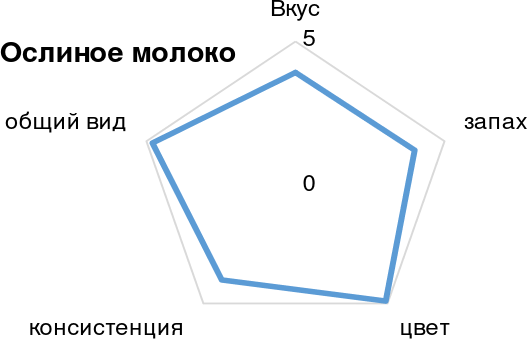
\includegraphics[width=0.5\textwidth]{assets/1106}
	\caption*{Рис.1- Профилограмма органолептических показателей ослиного молока}
\end{figure}

\begin{table}[H]
\caption*{Таблица 1 - Показатели безопасности ослиного молока}
\centering
\begin{tabular}{|p{0.15\textwidth}|p{0.1\textwidth}|p{0.15\textwidth}|p{0.15\textwidth}|p{0.2\textwidth}|}
\hline
Определяемые показатели & Ед.изме-рения & Допустимые значения (ТР ТС 021/2011) & Результаты испытаний & НД на методы испытаний \\ \hline
1 & 2 & 3 & 4 & 5 \\ \hline
Кадмий & мг/дм & 0,03 & \textless{}0,0015 & ГОСТ 33824-2016 \\ \hline
Свинец & мг/дм & 0,1 & \textless{}0,01 & ГОСТ 33824-2016 \\ \hline
Ртуть & мг/дм & 0,005 & \textless{}0,0037 & ГОСТ 26927-86 \\ \hline
Мышьяк & мг/дм & 0,05 & \textless{}0,04 & ГОСТ 31628-2012 \\ \hline
Афлатоксин М1 & мг/кг & \textless{}0,0005 & \textless{}0,0005 & ГОСТ 30711-2001 \\ \hline
Пестициды, в т.ч. &  & \multirow{2}{*}{\textless{}0,05} & \multirow{2}{*}{\textless{}0,04} & \multirow{3}{*}{МУ 2142-80 ч.11 М.815} \\ \cline{1-2}
α-ГХЦГ & \multirow{2}{*}{мг/кг} &  &  &  \\ \cline{1-1} \cline{3-4}
β-ГХЦГ &  & \textless{}0,05 & \textless{}0,04 &  \\ \hline
γ-ГХЦГ & \multirow{2}{*}{мг/кг} & \textless{}0,05 & \textless{}0,04 &  \\ \cline{1-1} \cline{3-5}
4,4'-ДДТ &  & \textless{}0,05 & \textless{}0,04 &  \\ \hline
4,4'-ДДД & мг/кг & не нормируется & \textless{}0,04 & \multirow{2}{*}{} \\ \cline{1-4}
4,4'-ДДЭ & мг/кг & не нормируется & \textless{}0,04 &  \\ \hline
Патогенная микрофлора в т.ч.сальмонеллы в 25,0 г продукта &  & не допускается & отсутствует & ГОСТ 31659-2012 \\ \hline
Listeria monocytogenes в 25,0 г продукта &  & не допускается & отсутствует & ГОСТ 32031-2012 \\ \hline
\end{tabular}
\end{table}

\begin{multicols}{2}
Анализ произведён по 5-ти балльной шкале. Среднее значение баллов по
всем характеристикам составило: внешний вид - 4,8; запах -- 4;
консистенция -- 4; вкус -- 3,9; цвет -- 4,9. Эксперты дали низкую
сенсорную оценку вкусу ослиного молока, что могло быть связано с высоким
содержанием сахара, придающим более сладковатый, не специфичный для
обычного молока вкус. Жидкая консистенция обусловлена низким содержанием
жира и высоким содержанием воды. Более высокий балл получил белоснежный
цвет молока, это могло быть связано с низким содержанием β-каротина.
Запах молока был оценён на 4 балла. Общая приемлемость ослиного молока
составила 4,32. Средние значения баллов в настоящем исследовании близки
значениям, указанным Malissiova {[}8{]}.

В санитарно-гигиенической лаборатории Центра государственного
санитарно-эпидемиологического надзора г. Бишкек получены результаты
анализа образцов ослиного молока по показателям безопасности (табл.1).

Приведённые в табл.1, результаты свидетельствуют о безопасности ослиного
молока, так как содержание афлатоксина М1, пестицидов и тяжёлых металлов
не превышает предельно допустимые нормы, установленные требованиями ТР
ТС 021/2011 «О безопасности пищевой продукции». Наличие соматических
клеток в молоке ослицы провели с препаратом «Мастоприм». По консистенции
исследуемое молоко характеризуется как однородная жидкость, за
деревянной палочкой тянется очень слабая нить, соответственно
показателям, количество соматических клеток менее 500 тыс. в 1 см3,
которая не превышает нормы безопасности {[}9-10{]}.

Физико-химические показатели молока ослиц кыргызской популяции в
сравнении с известными данными, представлены в табл.2., по каждому
показателю молока ослиц кыргызской популяции были проведены три пробы.
\end{multicols}

\begin{table}[H]
\caption*{Таблица 2 - Химический состав исследуемого ослиного молока}
\centering
\resizebox{\textwidth}{!}{%
\begin{tabular}{|l|l|l|l|l|l|l|l|}
\hline
Показатели & 1 проба & 2 проба & 3 проба & Ср.зна-чение & Polidori {[}15{]} & Salari {[}16{]} & Guo {[}17{]} \\ \hline
Массовая доля жира, \% & 0,5 & 0,6 & 0,5 & 0,5 & 0,3-1,8 & 0,46 & 1,16 \\ \hline
Массовая доля лактозы, \% & 6,2 & 6,2 & 6,3 & 6,2 & 5,8-7,4 & 6,83 & 6,33 \\ \hline
Массовая доля белка, \% & 1,7 & 1,7 & 1,7 & 1,7 & 1,5-1,8 & - & - \\ \hline
Титруемая кислотность, оТ & 5 & 5 & 5 & 5 &  & - & - \\ \hline
Плотность, Ао & 30 & 30 & 30 & 30 & - & - & - \\ \hline
Активная кислотность, рН & 7,3 & 7,4 & 7,3 & 7,3 & 7,0-7,2 & 7,2 & 7,18 \\ \hline
Сухие вещества, \% & 9,383 & 8,35 & 9,375 & 9,004 & 8,8-9,7 & 9,73 & 9,53 \\ \hline
\end{tabular}
}
\end{table}

\begin{multicols}{2}
Как видно из табл.2, показатели химического состава молока ослицы из с.
Беш-Кунгей схожи с показателями ранее исследуемых работ. Среднее
содержание массовой доли жира приближен к показателям итальянских
ученых, но меньше чем в молоке китайских ослиц, при этом содержание
лактозы во всех образцах сравнительно одинаковые.

Благодаря наличию природных антимикробных компонентов, таких как лизоцим
и лактоферрин, ослиное молоко обладает более длительным сроком годности
по сравнению с некоторыми другими видами молока. Эти компоненты помогают
предотвращать рост бактерий, что важно для хранения и транспортировки.
Термоустойчивость молока определяется его способностью выдерживать
высокие температуры без осаждения белков. Эта способность характеризует
технологичность молока, т.е. пригодность к последующей переработке. Для
определения термоустойчивости ослиного молока была использована
алкогольная проба в соответствии с ГОСТ 25228-82 {[}11{]}. Анализ
провели при помощи водного раствора этилового спирта с различной
объёмной концентрацией (68, 70, 72, 75, 80\%). По результатам
алкогольной пробы установлено, что исследуемое молоко устойчиво при
температуре 70-75 \textsuperscript{о}С. Вероятно, высокое содержание
сывороточных белков, а также сравнительно высокое содержание кальция
относительно казеинат-кальций-фосфатного комплекса является основной
причиной низкой термоустойчивости ослиного молока, что подтверждается
результатами исследования группы китайских учёных {[}14{]}, которые
установили, что при высоких температурах в ослином молоке наблюдается
седиментация. Оптимальными режимами пастеризации считаются: температура
63-65 ℃ с выдержкой 30 мин и 72-75 ℃ с выдержкой 15-20 мин {[}12-14{]}.

{\bfseries Выводы.} Ослиное молоко по своему составу близко к женскому
грудному молоку. Оно содержит высокий уровень лактозы и высокое
количество сывороточных белков, включая важные иммуноглобулины. Это
делает его потенциально полезным для детей, особенно для тех, кто не
переносит коровье молоко. Ослиное молоко имеет естественно низкую
жирность, что влияет на его консистенцию. Низкое содержание жира делает
его менее вязким по сравнению с коровьим молоком, что может быть полезно
для определенных пищевых продуктов и напитков, где требуется более
легкая текстура. Сенсорные показатели молока свидетельствуют о его
относительно приемлемом качестве, которое отличается сладким вкусом и
белоснежным цветом с голубоватым оттенком.

Результаты исследования показывают, что ослиное молоко может быть
перспективным компонентом для создания новых функциональных
(специальных) продуктов.
\end{multicols}

\begin{center}
{\bfseries Литература}
\end{center}

\begin{noparindent}
1.Турганбаева Н. Физиологически функциональные компоненты ослиного
молока // Знание. Развитие науки в XXI веке: сб. материалов междун.
научно-практ. конф. --Харьков, 2016. -№ 7-1 (36). - С. 48-54.

2. Taghiloo S., Allahmoradi E., Sadeghian-Kiadehi SF., Omrani-Nava V.,
Nazar E., Ebrahimzadeh MA. Up-regulation of human immune system function
by donkey's milk. //Brazilian Journal of Pharmaceutical Sciences. -
2020. -Vol. 56(7). DOI 10.1590/s2175-97902019000418449

3. Tafaro A. Immunological Properties of Donkeys Milk: Its Potential Use
in the Prevention of Atherosclerosis / T. Magrone, F. Jirillo, G.
Martemucci, A.G. D`Alessandro, L. Amati and E. Jirillo // Current
Pharmaceutical Design. -- 2007. -- Vol. 13. --P. 3711-3717.
DOI:10.2174/138161207783018590

4. Sarti L. Donkey's Milk in The Management of Children With Cow's Milk
Protein Allergy: Nutritional and Hygienic Aspect / L. Sarti, M. Martini,
G. Brajon, S. Barni, F. Salari {[}et al.{]} // Italian J. Pediatr. --
2019. -- Vol.: 45(1). DOI 10.1186/s13052-019-0700-4.

5. Altomonte L. Donkey and Human Milk: Insights into their Compositional
Similarities /\\
L. Altomonte, F. Salary, R. Licitra, M. Martini // International Dairy
Journal. - 2019. - Vol. 89. - P. 111-118. DOI
10.1016/j.idairyj.2018.09.005{\bfseries .}

6. Ellinger S. The effect of mare's milk consumption on functional
elements of phagocytosis of human

neutrophilsgranulocytes from healthy
volunteers / S. Ellinger, K.P. Linscheid, S. Jahnecke, R. Goerlich, H.
Endbergs // Food Agric Immunol. -2002. -Vol.: 14(3). - Р. 191-200. DOI
10.1080/09540100220145000b

7. Prasad B. Nutritional and Health Benefits of Donkey Milk // J Food
Science Nutritional Therapy. -- 2020. -- Vol. 6(1). -- P. 22-25. DOI
10.17352/jfsnt.000022.

8. Jirillo F. Donkey's and goat's milk consumption and benefits 311 to
human health with special reference to the inflammatory status / F.
Jirillo, E. Jirillo, T. Magrone // Curr Pharm Design. -- 2010. --Vol.:
16(7). -- Р. 859-863. DOI 10.2174/138161210790883688

9. Malissiova E. Assessment of Donkey Milk Chemical, Microbiological and
Sensory Attributes in Greece and Cyprus / E. Malissiova, G. Arsenos, Ph.
Papademas, D. Fletouris, A. Manouras, M. Aspri, A. Nikolopoulou, A.
Giannopoulou, I.S Arvanitoyannis // International J. of Dairy
Technology. - 2015. - Vol. 68. - P. 143-146. DOI
10.1111/1471-0307.12245.

10. ГОСТ Р 54077-2010. Методы определения соматических клеток по
изменению вязкости. -- Введ. 2010.30.11. -- М.: Стандартинформ, 2011. --
12 с.

11. ГОСТ 25228-82. Метод определения термоустойчивости по алкогольной
пробе. -- Введ. 26.04.1982, Переиздание 2008. Межгосударственный
стандарт. -- Москва: Стандартинформ, 2001. -- 4 с.

12. Luo J. Thermal Instability and Characteristics of Donkey Casein
Micelles / J. Luo, Sh. Jian, P. Wang, F. Ren, F. Wang, Sh. Chen, H. Gua
// Food Research International. -- 2019. -- Vol. 119. -- PP. 436-443.
DOI 10.1016/j.foodres.2019.02.023.

13. Salari F. A Multi-Approach Study of the Performance of Dairy Donkey
During Lactation: Preliminary Results / F. Salari, R. Ciampolini, C.
Mariti, F. Millanta, I. Altomonte, R. Licitra, B. Auzino, C. D' Ascenzi,
C. Bibbiani, L. Giuliotti, R. Amerigo Papini \& Mina Martini // Italian
Journal of Animal Science. - 2019. -Vol. 18(1). -P. 1135-1141. DOI
10.1080/1828051X.2019.1623094.

14. Guo H. Composition, Physiochemical Properties, Nitrogen Fraction
Distribution and Amino Acid Profile of Donkey Milk / H. Guo, K. Pang, X.
Zhang, L. Zhao, S.W. Chen, M.L. Dong, F.Z. Ren // Journal of Dairy
Science. -- 2007. -- Vol. 90, N 4. -- Р. 1635-1643. DOI
10.3168/jds.2006-600
\end{noparindent}
\newpage
\begin{center}
{\bfseries References}
\end{center}

\begin{noparindent}
1. Turganbaeva N. Fiziologicheski funktsional\textquotesingle nye
komponenty oslinogo moloka // Znanie. Razvitie nauki v XXI veke: sb.
materialov mezhdun. nauchno-prakt. konf. Khar\textquotesingle kov.-
2016. -№ 7-1 (36). - S. 48-54. {[}in Russian{]}

2. Taghiloo S., Allahmoradi E., Sadeghian-Kiadehi SF., Omrani-Nava V.,
Nazar E., Ebrahimzadeh MA. Up-regulation of human immune system function
by donkey's milk. //Brazilian Journal of Pharmaceutical Sciences.-
2020.-Vol. 56(7). DOI 10.1590/s2175-97902019000418449

3. Tafaro A. Immunological Properties of Donkeys Milk: Its Potential Use
in the Prevention of Atherosclerosis / T. Magrone, F. Jirillo, G.
Martemucci, A.G. D`Alessandro, L. Amati and E. Jirillo // Current
Pharmaceutical Design. -- 2007. -- Vol. 13. - 3711-3717.
DOI:10.2174/138161207783018590

4. Sarti L. Donkey's Milk in The Management of Children With Cow's Milk
Protein Allergy: Nutritional and Hygienic Aspect / L. Sarti, M. Martini,
G. Brajon, S. Barni, F. Salari {[}et al.{]} // Italian J. Pediatr. --
2019. -- Vol.: 45(1). -- P. 102. DOI:10.1186/s13052-019-0700-4.

5. Altomonte L. Donkey and Human Milk: Insights into their Compositional
Similarities /\\
L. Altomonte, F. Salary, R. Licitra, M. Martini // International Dairy
Journal. - 2019. - Vol. 89. - P. 111-118. DOI
10.1016/j.idairyj.2018.09.005{\bfseries .}

6. Ellinger S. The effect of mare's milk consumption on functional
elements of phagocytosis of human

neutrophilsgranulocytes from healthy
volunteers / S. Ellinger, K.P. Linscheid, S. Jahnecke, R. Goerlich, H.
Endbergs // Food Agric Immunol. -- 2002. -- Vol.: 14(3). -- Р. 191-200.
DOI 10.1080/09540100220145000b

7. Prasad B. Nutritional and Health Benefits of Donkey Milk // J Food
Science Nutritional Therapy. -- 2020. -- Vol. 6(1). -- P. 22-25. DOI
10.17352/jfsnt.000022.

8. Jirillo F. Donkey's and goat's milk consumption and benefits 311 to
human health with special reference to the inflammatory status / F.
Jirillo, E. Jirillo, T. Magrone // Curr Pharm Design. -- 2010. --Vol.:
16(7). -- Р. 859-63. DOI: 10.2174/138161210790883688

9. Malissiova E. Assessment of Donkey Milk Chemical, Microbiological and
Sensory Attributes in Greece and Cyprus / E. Malissiova, G. Arsenos, Ph.
Papademas, D. Fletouris, A. Manouras, M. Aspri, A. Nikolopoulou, A.
Giannopoulou, I. S Arvanitoyannis // International J. of Dairy
Technology. -- 2015. -- Vol. 68. -- P. 143-146. DOI
10.1111/1471-0307.12245.

10. GOST R 54077-2010. Metody opredeleniya somaticheskikh kletok po
izmeneniyu vyazkosti. -- Vved. 2010.30.11. -- M.: Standartinform, 2011.
-- 12 s. {[}in Russian{]}

11. GOST 25228-82. Metod opredeleniya termoustoichivosti po
alkogol\textquotesingle noi probe. -- Vved. 26.04.1982, Pereizdanie
2008. Mezhgosudarstvennyi standart. -- Moskva: Standartinform, 2001. --
4 s. {[}in Russian{]}

12. Luo J. Thermal Instability and Characteristics of Donkey Casein
Micelles / J. Luo, Sh. Jian, P. Wang, F. Ren, F. Wang, Sh. Chen, H. Gua
// Food Research International. -- 2019. -- Vol. 119. -- PP. 436-443.
DOI 10.1016/j.foodres.2019.02.023.

13. Salari F. A Multi-Approach Study of the Performance of Dairy Donkey
During Lactation: Preliminary Results / F. Salari, R. Ciampolini, C.
Mariti, F. Millanta, I. Altomonte, R. Licitra, B. Auzino, C. D' Ascenzi,
C. Bibbiani, L. Giuliotti, R. Amerigo Papini \& Mina Martini // Italian
Journal of Animal Science. -- 2019. -- Vol.18:1. -- P. 1135-1141. DOI
10.1080/1828051X.2019.1623094.

14. Guo H. Composition, Physiochemical Properties, Nitrogen Fraction
Distribution and Amino Acid Profile of Donkey Milk / H. Guo, K. Pang, X.
Zhang, L. Zhao, S.W. Chen, M.L. Dong, F.Z. Ren // Journal of Dairy
Science. -- 2007. -- Vol. 90, N 4. -- Р. 1635-1643. DOI
10.3168/jds.2006-600
\end{noparindent}

\emph{{\bfseries Сведения об авторах}}

\begin{noparindent}
Турганбаева Н.К. -- ст. преподаватель Кыргызско-Турецкого университета
``Манас'', Бишкек, Кыргызстан, e-mail: nadira.turganbaeva@manas.edu.kg;

Элеманова Р.Ш. - к.т.н., доцент, проректор по академической работе
Кыргызского государственного технического университета им. И. Раззакова,
Бишкек, Кыргызстан; e-mail: elemanova@kstu.kg;

Дюшеева Н.С. - аспирант Кыргызского государственного технического
университета им. И. Раззакова, Бишкек, Кыргызстан, e-mail:
nurguloo@mail.ru.
\end{noparindent}

\emph{{\bfseries Information about the author}}

\begin{noparindent}
Turganbaeva N.K. - Senior Lecturer, Kyrgyz-Turkish University "Manas",
Bishkek, Kyrgyzstan, e-mail: nadira.turganbaeva@manas.edu.kg;

Elemanova R.Sh. - Candidate of Technical Sciences, Associate Professor,
Vice-Rector for Academic Work, Kyrgyz State Technical University named
after I. Razzakov, Bishkek, Kyrgyzstan, e-mail: elemanova@kstu.kg;

Dyusheeva N.S. - Рost-graduate student, Kyrgyz State Technical
University named after I. Razzakov, Kyrgyzstan, e-mail:
nurguloo@mail.ru.
\end{noparindent}
